\chapter{Teoretická část}\label{chap:teorie}

Tato kapitola budu věnována přiblížení teoretického kontextu této práce.

\section{Virtualizace}

Koncept virtualizace se poprvé objevil na konci 50.\,let minulého století, kdy skupina z University v Manchesteru vytvořila první funkční prototyp virtuální paměti. Následně v 60.\, letech minulého století byl koncept rozšířen i na celé počítače. První tzv. \textit{virtual machine} (VM), neboli česky \uv{virtuální stroj}, byl vytvořen firmou IBM a jeho cílem bylo umožnit souběžný přístup k sálovým počítačům. Každá VM byla instancí fyzického stroje a dávala iluzi toho, že uživatel přistupuje přímo k fyzickému stroji. Uživatelé mohli vyvíjet, spouštět a testovat aplikace bez obavy toho, že by mohli zhroutit celý počítač, díky tomu, že každá VM byla izolovanou kopií systému. 

V polovině 70.\,let minulého století byla virtualizace již dobře akceptovaným konceptem mezi uživateli. Použitím virtualizace totiž mohli vyřešit podstatné problémy této doby. Například díky již zmíněné virtualizované paměti mohli uživatelé adresovat mnohem větší operační paměť, než počítač skutečně obsahoval. 

Všechny tyto virtualizační techniky byly primárně cestou k vyrovnání se s vysokou pořizovací cenou hardwaru v této době. Díky ní mohli majitelé sálových počítačů využít svoji investici co nejefektivněji. Její použití se tedy se snižujícími cenami hardwaru začalo snižovat a dokonce skoro vymizelo během 80. a 90.\,let díky příchodu levnějších osobních počítačů.  

Poptávka po virtualizaci začala znovu růst až v 90.\,letech minulého století. Se zvětšující se různorodostí hardwaru a softwaru zde vznikla poptávka na schopnost spustit aplikace, které původně byly určeny pro jiný hardware a jiný operační systém, na jednom určitém stroji. 

Poptávka se ovšem zvětšila i v komerčním sektoru. S zvyšujícími se počty serverů firmy hledaly způsoby, jak využít tuto investici do serveru naplno. Spustit pouze jednu aplikaci na serveru nebylo příliš ekonomické, jelikož tato aplikace nemusela vždy využít všechny výpočetní zdroje, a nákup dalších serverů přinášel mimo samotné pořizovací ceny i další náklady, například na údržbu a administraci. Řešením pro tento problém byla opět virtualizace. Oba tyto trendy pokračují do dnes a jsou jedny z hlavních důvodů pro dnešní využití virtualizace. 

Virtualita se od reality liší pouze ve formálním světě. Má ovšem podobné jádro nebo efekt. V počítačovém světě je virtualizované prostředí vnímáno aplikací stejně jako reálné prostředí, i když některé mechanismy v něm mohou fungovat jinak. Toto prostředí hlavně dává aplikaci zkreslený obraz reálného stroje, kde v tomto zkresleném obraze může stroj mít více, či méně určitých zdrojů. Typický moderní počítač využívá spoustu takovýchto přístupů. Jedním příkladem je již zmíněná virtuální paměť, díky čemuž může proces použít mnohem více paměti, než je fyzicky dostupné. Tato virtuální paměť taktéž umožňuje sdílení fyzické paměti mezi stovkami procesy. Podobným konceptem je i multitasking, kde jeden procesor je rozdělen a prezentován jako \uv{virtuální procesor} jednotlivým procesům. Na druhou stranu, několik procesorů může být seskupeno do jednoho výkonnějšího virtuálního procesoru.

Možností virtualizace je tedy spousta na mnoha úrovních. Virtualizaci tedy můžeme nadefinovat takto:

\begin{displayquote}
    Virtualizace je technologie, která kombinuje/rozděluje, výpočetní zdroje k prezentaci jednoho či více prostředí za pomoci metodologií jako hardwarového a softwarového rozdělování/agregování, parciální/kompletní simulací stroje, emulace a spousty dalších.
\end{displayquote}

Jak je z definice vidět, virtualizace není jenom o rozdělování výpočetních zdrojů, ale i o jejich sjednocování do větších celků. V rámci této práce se ale zaměřím primárně na rozdělování výpočetních zdrojů za pomoci virtualizace. Mezi praktické využití virtualizace může patřit například:

\begin{description}
    \item[Konsolidace serveru] Za pomoci virtualizace lze přerozdělit práci z více serverů, které nejsou na plno používány, na jeden server a tím ušetřit na hardwaru, managmentu a administraci infrastruktury. Díky ní tedy snižujeme komplexitu administrace, jelikož všechen software ve VM je nezávislý na softwaru fyzického serveru. 
    \item[Sandbox] Za pomoci virtualizace lze vytvořit bezpečné a hlavně izolované prostředí pro běh aplikací, jejichž původ nám může být neznámý a spuštění v normálním prostředí počítače by mohlo představovat bezpečnostní riziko. Tato technika se označuje jako \textit{sandboxing}.
    \item[Virtuální hardware] Virtualizace může zprostředkovat hardware, který počítač nikdy neměl. Mezi ně patří například virtuální ethernetové adaptéry, switche, huby atd.
    \item[Spuštění více OS] Bez virtualizace nejsme schopni spustit více operačních systémů zároveň. Virtualizace tedy přináší prostředky, jak toto umožnit. Mimo to ale také přináší prostředky, jak spustit staré operační systémy na novém hardwaru, pro který daný operační systém nemusel být vyvinut.
    \item[Testování/QA] S pomocí virtualizace jsme schopni vytvořit libovolné testovací scénáře, které jinak mohou těžké vytvořit v reálném světě, čímž může usnadnit testování. 
\end{description}

Jak je vidět z jenom z tohoto krátkého seznamu, důvodů proč virtualizovat existuje spousta. Jak ale virtualizace funguje? V praxi je virtualizace abstrakční vrstva, která poskytuje potřebné propojení mezi dvěma izolovanými vrstvami. Toto si lze lépe představit pomocí obrázku \ref{fig:pc_stack}, na kterém je vidět zjednodušená architektura počítače. Je zde vidět, že virtualizační vrstvu lze vložit mezi jakékoliv dvě vrstvy a tím docílit virtualizace. \cite{campbell2006introduction}\cite{chiueh2005survey}

\begin{figure}[htbp]
    \centering 
    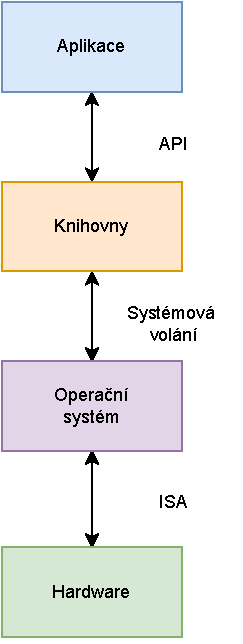
\includegraphics[width=0.325\textwidth]{assets/img/computer_stack.pdf}
    \caption{Architektura počítače ukazující příležitosti k virtualizaci}
    \source{Vytvořeno dle předlohy z \cite{chiueh2005survey}}
    \label{fig:pc_stack}
\end{figure}

V případě dnes nejpopulárnější architektury x86 je potřeba i rozlišit, s jakými právy daná virtualizace běží. Architektura x86 definuje tzv. \textit{protekční kruhy}, kde každý kruh(anglicky se tyto úrovně označují jako \textit{ring}), neboli úroveň, definuje, co daná aplikace může a nemůže udělat. Grafickou představu těchto úrovní můžeme vidět na obrázku \ref{fig:priv_rings}. Jak je vidět, čím nižší úroveň, tím více práv aplikace běžící v této úrovni má. Typicky, v úrovni 0 běží operační systém a aplikace následně běží v úrovni 3. \cite{RODRIGUEZHARO2012267}

\begin{figure}[htbp]
    \centering 
    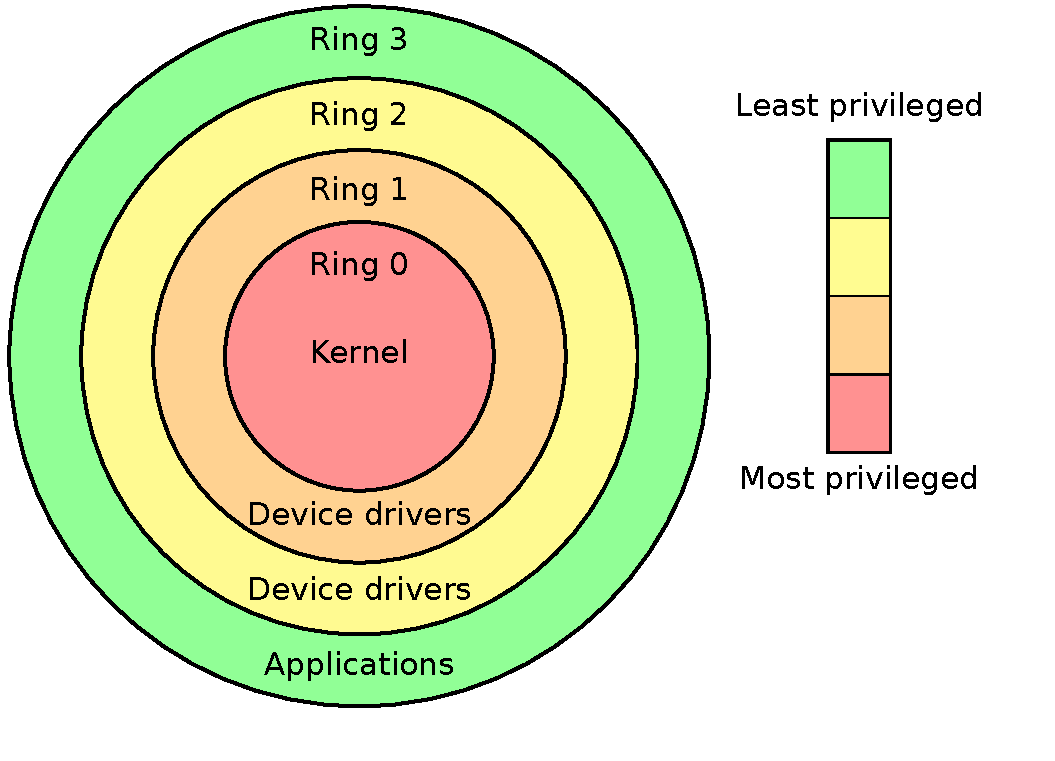
\includegraphics[width=\textwidth]{assets/img/priv_rings.pdf}
    \caption{Architektura počítače ukazující příležitosti k virtualizaci}
    \source{Wikipedia Commons \cite{privrings}}
    \label{fig:priv_rings}
\end{figure}

\subsection{Hypervizor}

Důležitou komponentou při virtualizaci je tzv. \textit{hypervizor} (někdy taky označován jako Virtual Machine Monitor - VMM). Hypervizor je softwarová vrstva, která virtualizuje všechny potřebné zdroje fyzického stroje, a tím definuje a podporuje běh jednoho či více VM. \cite{whitaker2002denali}

Existují dva typy hypervizorů. Ty můžeme vidět na obrázku \ref{fig:vm_types}. Hypervizor typu I běží přímo nad hardwarem a spravuje všechny virtuální stroje. Díky tomu hypervizor může mít plnou kontrolu nad hardwarem, jelikož běží v úrovni nejvyšší priority. Hypervizor typu 2 běží nad hostitelským operačním systém, respektive uvnitř něj. Tento hypervizor je odkázán na hostitelský systém, který mu přiděluje prostředky, jelikož každá VM je v podstatě další proces v systému.\cite{chiueh2005survey}\cite{RODRIGUEZHARO2012267}

\begin{figure}[htbp]
    \centering 
    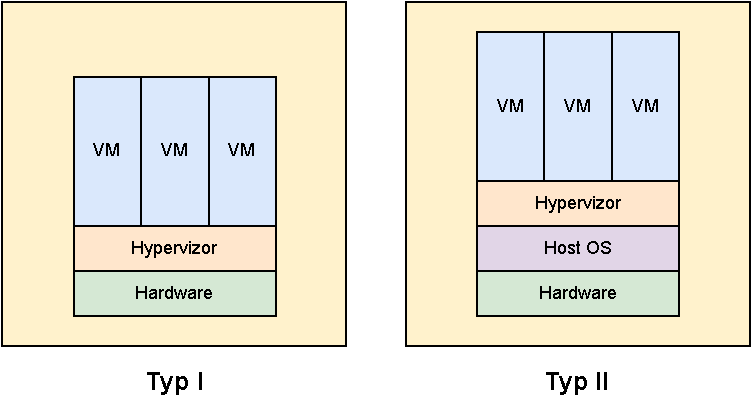
\includegraphics[width=\textwidth]{assets/img/vm_types.pdf}
    \caption{Možné typy virtualizace na úrovni HAL}
    \source{Vytvořeno dle předlohy z \cite{RODRIGUEZHARO2012267}}
    \label{fig:vm_types}
\end{figure}

\subsection{Možnosti virtualizace z technologického pohledu}

Jak již bylo nastíněno, virtualizační vrstva může existovat na více úrovních. V této sekci bude přiblížena virtualizace od nejnižší vrstvy až po tu nejvyšší.

\subsubsection{Virtualizace ISA}

ISA, neboli \textit{Instruction Set Architecture} je součástí abstraktního modelu počítače a definuje, jak může software ovládat procesor. ISA funguje jako rozhraní mezi hardwarem a softwarem a specifikuje, co a jak je procesor schopen udělat.\,\cite{isa-arm}

Virtualizace na této úrovni tedy funguje za pomoci softwarové emulace ISA dané platformy. Tedy virtuální vrstva musí být schopna přeložit ISA instrukce hosta na na ISA instrukce hostitele. Tento způsob lze označit i jako \textit{binární překlad}. Tato virtualizace funguje pouze v případě, že existuje způsob, jak na hostitelské platformě provést všechny úkony, požadované architekturou hosta. 

Výhodou této virtualizace je, že nám teoreticky dokáže dát dostatečné prostředky ke spuštění jedné platformy (jako například x86) na ostatních platformách. Taktéž jsme schopni spustit operační systémy, bez žádné modifikace. Tato portabilita ovšem přichází s nemalou cenou. Tím, že musíme každou instrukci softwarově přeložit, tak dochází k velkému snížení výkonu systému. I tak si tento způsob virtualizace nalezne využití. \cite{chiueh2005survey}\cite{RODRIGUEZHARO2012267}


\subsubsection{Virtualizace HAL}

Hardware abstraction layer (HAL), neboli česky hardwarová abstrakční vrstva, je vrstva, která vytváří jednotné API pro přístup k hardwaru. Díky němu je možné oddělit implementaci přístupu k hardwaru od samotného softwaru. Software totiž pouze využívá API definované HAL a až následná implementace na daném zařízení definuje reálný přístup k hardwaru daného stroje. \cite{haldef}

Virtualizace HAL tedy využívá podobnosti mezi architekturou platformy hosta a hostitele, díky čemuž je snížena latence způsobená překladem. Často je ovšem spojována společně s binárním překladem. Ten může nastat například z důvodu nedostatečných práv k vykonání operace, v rámci úrovně ve které hypervizor běží. \cite{chiueh2005survey}\cite{vcc_2}


\subsubsection{Virtualizace na úrovni programovacího jazyka}

Virtualizace na úrovni programovacího jazyka probíhá v rámci aplikační vrstvy. Ideou bylo, vytvořit virtuální stroj již na aplikační úrovni, který oddělí aplikaci od hardwaru. Implementace tohoto aplikačního virtuálního stroje následně definuje reálný přístup k výpočetním zdrojů. K těm je přistupováno standardizovaným způsob, jenž je definován abstrakční vrstvou. Pro představu lze uvést například Java Virtual Machine, nebo Common Language Runtime v .NET Frameworku. \cite{chiueh2005survey}


\subsubsection{Virtualizace na úrovni knihoven}

Virtualizace na úrovni knihoven může připomínat předchozí popsanou virtualizaci, ovšem důležitá je změna původu této implementace. Každá aplikace využívá volání různých externích zdrojů. Tyto zdroje mohou a nemusí být přenositelné mezi operačními systémy. Virtualizace na této úrovni využívá rozhraní daných externích zdrojů, ale ovšem implementace je přizpůsobena tomu stroji, na kterém aplikace běží. Jako příklad můžu uvést například Wine, který implementuje Windows API v UNIX prostředí. 


\subsection{Virtualizační techniky}

V následující sekci jsou přiblíženy reálné přístupy k virtualizaci, které používají buď jednu z předem zmíněných virtualizačních technik, nebo tyto techniky kombinují. 

\subsubsection{Plná virtualizace}

Plná virtualizace funguje na principu kombinace přímého spuštění instrukcí a binárního překladu instrukcí za běhu. Využívá se toho, že hypervizor běží na nulté úrovni, tedy s nejvyšší prioritou a s největšími právy. Hypervizor tím pádem zcela odděluje operační systém od skutečného hardwaru. Toto lze vidět na obrázku \ref{fig:full_virt}.\cite{4709159}

\begin{figure}[htbp]
    \centering 
    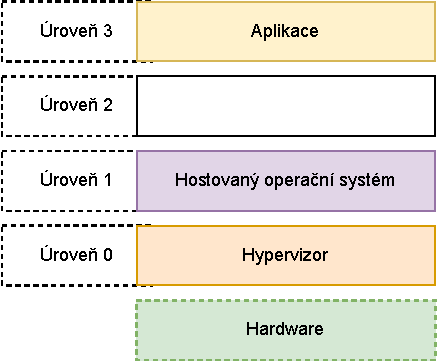
\includegraphics[width=0.65\textwidth]{assets/img/full_virt.pdf}
    \caption{Plná virtualizace}
    \source{Podle \cite{vcc_2}}
    \label{fig:full_virt}
\end{figure}


\subsubsection{Paravirtualizace}

Paravirtualizace funguje na stejných úrovních jako plná virtualizace. Hypervizor má plnou kontrolu nad hardwarem hostitelského stroje a operace s ním jsou zprostředkovávány hypervizorem. Změna ovšem nastává v rámci operačního systému. Ten má totiž upravené jádro a díky tomu ví, že běží v paravirtualizovaném prostředí. Jednotlivá ISA volání jsou tedy nahrazena voláním virtualizačních funkcích. Tedy operační systém přímo komunikuje s hypervizorem.\cite{4709159}


\subsubsection{Hardwarově asistovaná virtualizace}

Hardwarově asistovaná virtualizace funguje na principu přímé podpory virtualizace ze strany hardwaru. V rámci této virtualizace je mezi protekční vrstvy přidána nová vrstva na úroveň -1, tedy pod všechny ostatní úrovně. Privilegované instrukce jsou tedy zachyceny přímo hardwarem a následně jsou předány hypervizoru ke zpracování.\cite{4709159}

\begin{figure}[htbp]
    \centering 
    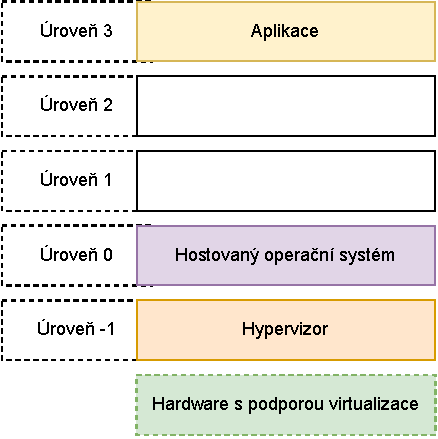
\includegraphics[width=0.65\textwidth]{assets/img/hardware-asssist-virt.pdf}
    \caption{Hardwarově asistovaná virtualizace}
    \source{Podle \cite{vcc_2}}
    \label{fig:hardware_asssist_virt}
\end{figure}

\subsubsection{Kontejnerová virtualizace}

Kontejnerová virtualizace, neboli zkráceně kontejnerizace, je lehčí alternativou k tradiční virtualizaci. Porovnání s tradiční virtualizací můžeme vidět na obrázku \ref{fig:containerization}. Tradiční VM jsou nahrazeny tzv. \textit{kontejnery}. Jak je vidět, kontejnery již nemusí obsahovat kopii celého operačního systému. Kontejnery totiž sdílí jádro operačního systému a další zdroje, jako například knihovny. Díky tomu mohou být spouštěny mnohem rychleji než VM. \cite{8693491}

Všechny kontejnery jsou následně orchestrovány tzv. \textit{kontejnerizátorem}, v angličtině \textit{container engine}. Ten má na starost vše spojené s procesem spouštění a běhu kontejneru. Díky němu je mimo jiné možné rychle a efektivně propojit kontejnery mezi sebou.\cite{Bentaleb2021} 

Nevýhodou kontejnerů je ovšem to, co je tvoří tak efektivními. Sdílením jádra může docházet k bezpečnostním rizikům, díky čemuž jsou méně bezpečné než tradiční VM.\cite{6498558}


\begin{figure}[htbp]
    \centering 
    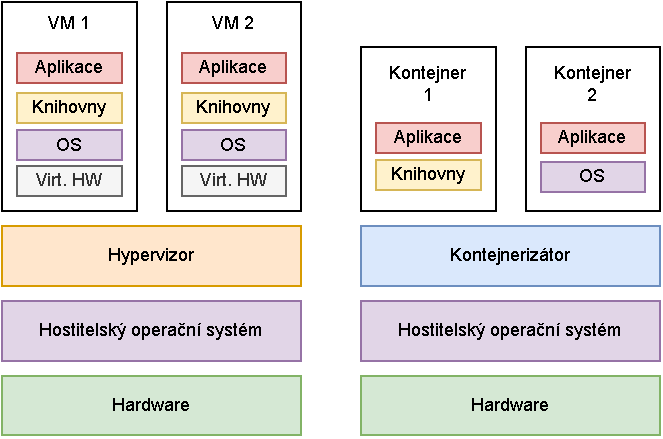
\includegraphics[width=0.9\textwidth]{assets/img/containerization.pdf}
    \caption{Porovnání virtualizace s hypervizorem oproti virtualizaci kontejnerizací}
    \source{Podle \cite{vcc_2}}
    \label{fig:containerization}
\end{figure}


\subsection{Virtualizační řešení}

V předchozí sekcích byly představeny možnosti jak lze virtualizovat. Následující sekce jsou věnované vybraným řešením, které dnes pro virtualizaci existují.


\subsubsection{VMware}

\subsubsection{QEMU}

\subsubsection{Docker} \customtodo{zmínit docker compose a dockefile}
Docker je neznámějším a nejrozšířenějším nástrojem, který zprostředkovává kontejnerizaci. Proto také ve většině případech je většina ostatních nástrojů s Docker srovnávaná. Docker se skládá z několika hlavních komponent, které dohromady tvoří námi požadovaný container engine. Mezi tyto komponenty patří

\begin{itemize}
    \item Docker Client and Server,
    \item Docker Containers,
    \item Docker Images,
    \item Docker Registries.
\end{itemize}

Docker Client and Server jak z překladu názvu vyplývá obsahuje klienta a server. Server dostává žádosti od klienta, které následně zpracovává. Architekturu nástroje Docker můžeme vidět na obrázku \ref{fig:docker_arch}. Zajímavou komponentou je Docker Daemon, což je persistentní proces, který neustále běží na pozadí. Klient provádí komunikaci s Docker Daemon prostřednictvím stanového REST API a ten se následovně stará o sestavování, běh a distribuci Docker kontejnerů. Docker server a klient může běžet na jednom stroji, ale zároveň klient se může k serveru připojit i vzdáleně. 
\cite{turnbull2014docker}\cite{docker_overview}

\begin{figure}[htbp]
    \centering 
    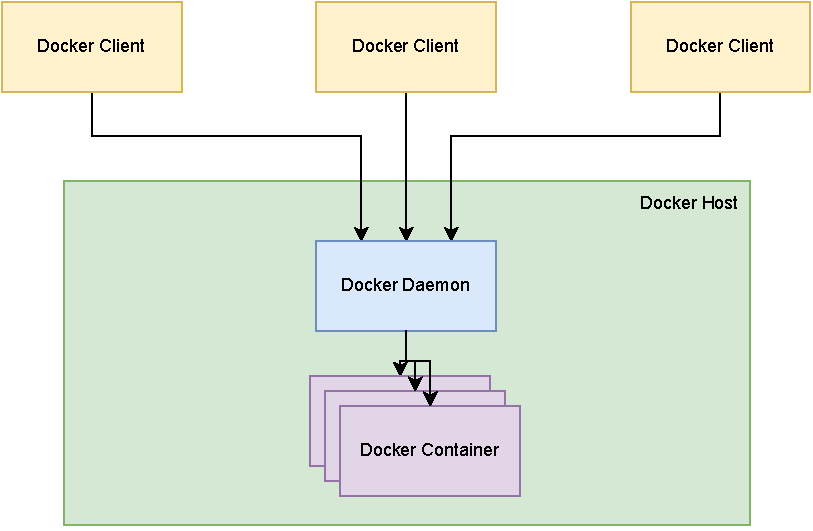
\includegraphics[width=0.97\textwidth]{assets/img/docker_arch.pdf}
    \caption{Docker architektura}
    \source{Vytvořeno dle předlohy z \cite{turnbull2014docker}}
    \label{fig:docker_arch}
\end{figure}

Jednotlivé Docker kontejnery jsou vytvářeny z tzv. Docker Images. Tyto images, neboli v češtině obrazy, obsahují definici všech závislostí a balíčků, potřebných k běhu kontejneru. Způsoby jak vytvářet obrazy jsou dva - buď můžeme definovat vlastní obraz a nebo použít nějakou již vytvořenou předlohu. Je podstatné zmínit, že každý existující obraz může být předlohou pro nový obraz. 

Tyto obrazy následně můžou být uloženy v Docker Registries. Ten slouží jako repositář pro obrazy, který může být buď veřejný, nebo soukromý. Veřejný repositář se nazývá Docker Hub, kde každý může získat kterýkoliv již vytvořený image, a nebo může také nahrát vlastní. \cite{turnbull2014docker} 

Docker v základu nabízí několik druhů síťových ovladačů. Síťový typ \textit{host} umožňuje odstranit izolaci mezi kontejnery a plně využít síť zprostředkovanou hostem, tedy Docker serverem. Oproti tomu síťový typ \textit{overlay} slouží k propojení různých Docker daemonů a umožňuje komunikace mezi nimi. 

Pro naše použití ale začínají být zajímavé až síťové typy \textit{bridge}, \textit{IPvlan} a \textit{MACvlan}. \textit{Bridge} je výchozím síťovým typem, který Docker používá v momentě kdy dva kontejnery potřebují mezi sebou komunikovat na stejném zařízení. \textit{IPvlan} oproti tomu umožňuje uživatelům plnou kontrolu nad IPv4 a IPv6 adresováním a nad druhou a třetí úrovní ISO/OSI modelu. V neposlední řadě \textit{MACvlan} umožňuje kontejnerům přiřadit různé MAC adresy, které tak mohou být odlišné od hostujícího zařízení. To umožňuje kontejnerům vypadat na síti jako fyzické zařízení.

Docker také podporuje vlastní implementace síťových ovladačů. Ty následně mohou být nahrány do stejného repositáře jako Docker obrazy. Bohužel jelikož tyto síťové ovladače jsou zahrnuty do širší kategorie \uv{rozšíření}, tak jejich vyhledávání je náročné a často neobsahují skoro žádný popis. \cite{docker_networking_overview}\cite{docker_brige_overview}

Díky tak širokému využití Docker je jeho podpora rozšířena i pro jazyk \csharp~díky knihovnám, které byly vytvořeny komunitou. Ty umožňují přímo sestavovat a nasazovat kontejnery a spravovat virtuální síť. To velice ulehčuje jeho možné použití v testovací knihovně. 

\subsubsection{Podman}
Podman je velice podobný Dockeru. Tento nástroj je primárně zaměřený na operační systém Linux, kde pomáhá najít, spustit a nasadit kontejnery dle pravidel OCI. V použití je dokonce až tak podobný, že většina uživatelů může změnit příkaz \inlinecode{docker} na \inlinecode{podman} bez problémů. Rozdíly tam ale přeci jen jsou. 

Podman oproti Docker používá takzvanou \textit{daemon-less} architekturu. Jak už bylo zmíněno, Docker obsahuje neustále běžící proces který se nazývá \textit{daemon}, který poslouchá příkazy od klienta a spravuje všechny procesy spojené s kontejnerizací. Tento přístup vytváří problémy hlavně z bezpečnostního hlediska, jelikož daemon musí být spuštěn s právy správce počítače. Docker sice podporuje od verze v19.03 tzv. \textit{rootless execution}, tedy mód kdy nepotřebuje práva správce, ale při chodu v tomto módu mohou uživatelé narazit na různé limitace.

A na toto se přesně zaměřil Podman. Podman používá pro správu kontejnerů nástroj \textit{systemd}, který ke spuštění využívá práva uživatele, který provádí příkazy. Podman také využívá jiný nástroj \textit{Buildah}, za pomocí něhož je schopen sestavovat kontejnery bez daemona. \cite{podman}\cite{podman_vs_docker}

Podman stejně jako Docker podporuje síťové typy \textit{bridge} a \textit{MACvlan}. Ovšem k jejich použití již potřebuje práva správce počítače. K vyřešení tohoto problému Podman používá síťový typ \textit{slirp4netns}. Ta vytvoří speciální TAP zařízení, fungující na linkové vrstvě ISO/OSI modelu a umožňuje komunikaci mezi kontejnery, které jsou ovšem takto fungují izolovaně od sebe. \cite{podman_network}

Jak jsem řekl na začátku, Podman je nástroj primárně zaměřený na operační systém Linux, ovšem má i svou distribuci pro Windows. Ovšem k tomu aby mohl na Windows fungovat, tak každý kontejner musí obsahovat hostující systém Linux, na kterém jsou následně kontejnery spuštěny. \cite{podman_vs_docker}

\subsubsection{Vagrant}

Vagrant je nástroj, který se primárně zaměřuje na to, aby přinesl konzistentní vývojové prostředí na různé operační systémy. Jeho hlavní výhodou oproti Docker je jeho široká podpora operačních systému, které Docker nepodporuje. 

Stejně jako Docker, i Vagrant má širokou podporu komunitních obrazů, ze kterých jsou následně vytvářeny tzv. \textit{boxy}, což je pouze jiný název pro kontejnery.\cite{vargrant_vs_docker}
\customtodo{Rozšířit}

V některých aspektech jsou ovšem ostatní možnosti lepší volbou. Jednou z nich je využití výpočetních zdrojů. Oproti Docker, který používá přímo zdroje hostujícího stroje, tak každá virtuální mašina vytvořená ve Vagrant spotřebuje specifický počet jáder, paměti RAM a paměti na disku. Zároveň čas změny konfigurace a sestavení virtuální mašiny je mnohem rychlejší na Docker, než ve Vagrant.\cite{madapparambath_2022}
\question{Nechat Vagrant nebo ne, jelikož co koukám tak to kontejnerizaci nedělá? Hledat náhradu?}
